%versi 2 (8-10-2016)-pppppppppppppp;
\chapter{Perancangan dan Implementasi}
\label{chap:perancanganDanImplementasi}
\setcounter{secnumdepth}{3}

\paragraph{}
\section{Perancangan Basis Data}
\subsection{Model Relasional}
Dari analisis yang telah dilakukan, maka dibuatlah model relasional seperti pada gambar 4.1

\begin{figure} [H]
	\centering  
	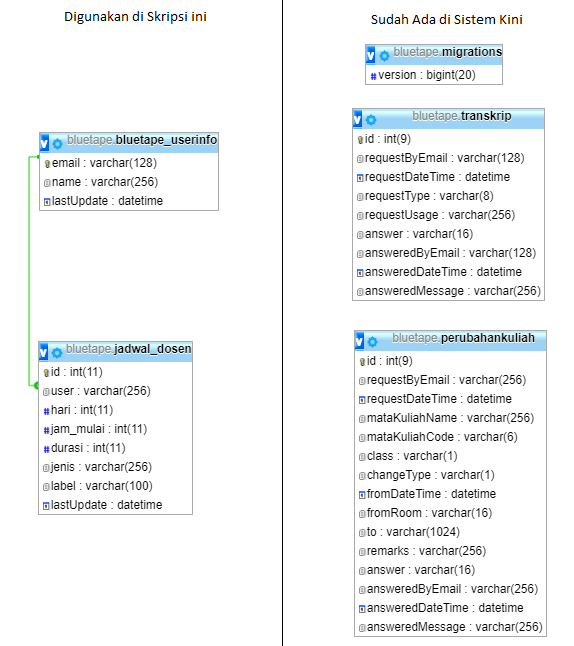
\includegraphics[scale=0.9]{ERDiagram.png}  
	\caption[Model Realsional]{Model Realsional} 
	\label{fig:skematik-phpexcel} 
\end{figure}

\subsection{Perancangan Tabel}
\begin{center}
	\begin{table}[H]
	\begin{tabular}{|c|c|c|c|c|c|c|}
 			\hline
		\textbf{Atribut} & \textbf{Tipe Data} & \textbf{Ukuran} & \textbf{Primary Key} & \textbf{Foreign Key} & \textbf{Null} & \textbf{Keterangan} \\
			\hline
		 id & int & 11 & ya & tidak & tidak & id jadwal\\
			 \hline
			 user & varchar & 256 & tidak & ya & tidak & pemilik jadwal\\
			 \hline
			 hari & int & 11 & tidak & tidak & tidak & hari berlangsungnya jadwal\\
			 \hline
			 jam\_mulai & int & 11 & tidak & tidak & tidak & jam berlangsungnya jadwal\\
			 \hline
			 durasi & int & 11 & tidak & tidak & tidak & lama jadwal berlangsung\\
			 \hline
			 jenis & varchar & 255 & tidak & tidak & tidak & jenis kegiatan jadwal\\
			 \hline
			 label & varchar & 100 & ya & tidak & tidak & nama kegiatan\\
			 \hline
	\end{tabular}
	\caption{Perancangan Tabel Jadwal}
	\end{table}
\end{center}

\subsection{Perancangan Rinci}
\subsubsection{Controller EntriJadwalDosen}
\paragraph{} Berikut adalah perancangan kelas Controller EntriJadwalDosen \\
\begin{tabular}{|c|p{11cm}|}
\hline
Nama Method 	& 	insert 	\\
\hline
Parameter Output & insert\_success, insert\_failed \\
\hline
Tabel yang berhubungan & jadwal\_dosen \\
\hline
Deskripsi	& Proses untuk memasukan jadwal \\
\hline
Algoritma	& \begin{itemize}
				\item proses menerima input-input data dari user
				\item proses mengecek apakah data-data yang dimasukan sudah valid
				\item proses mengecek apakah jadwal yang bertabrakan dengan jadwal lain atau tidak
				\item bila jadwal bertabrakan dengan jadwal lain maka proses menampilkan pesan "Jadwal gagal dimasukan. Sudah ada jadwal lain pada waktu ini"
				\item bila tidak ada masalah , proses akan memasukan data ke dalam database
				\end{itemize} \\
\hline
\end{tabular}
\\

\begin{tabular}{|c|p{11cm}|}
\hline
Nama Method 	& 	edit 	\\
\hline
Parameter Output & edit\_success, edit\_failed \\
\hline
Tabel yang berhubungan & jadwal\_dosen \\
\hline
Deskripsi	& Proses untuk mengubah jadwal yang sudah dimasukan sebelumnya \\
\hline
Algoritma	& \begin{itemize}
				\item proses menerima input-input data dari user
				\item proses mengecek apakah data-data yang dimasukan sudah valid
				\item proses mengecek apakah waktu baru dari jadwal yang diubah bertabrakan dengan jadwal lain atau tidak
				\item bila jadwal bertabrakan dengan jadwal lain maka proses menampilkan pesan "Pengubahan gagal. Sudah ada jadwal lain pada waktu ini"
				\item bila tidak ada masalah, maka jadwal akan memperbarui data yang ada di database.
				\end{itemize} \\
\hline
\end{tabular}
\\

\begin{tabular}{|c|p{11cm}|}
\hline
Nama Method 	& 	delete 	\\
\hline
Parameter Output & deleted \\
\hline
Tabel yang berhubungan & jadwal\_dosen \\
\hline
Deskripsi	& Proses untuk menghapus jadwal \\
\hline
Algoritma	& \begin{itemize}
				\item proses menerima pilihan jadwal yang akan dihapus oleh user.
				\item proses mengeluarkan form konfirmasi untuk memastikan user untuk menghapus jadwal yang bersangkutan
				\item bila user memilih "ya", maka data jadwal yang bersangkutan akan dihapus dari database.
				\item bila pilihan user "tidak" maka proses akan menampilkan halaman sebelum user menekan tombol \textit{delete}.
				\end{itemize} \\
\hline
\end{tabular}


\subsubsection{Controller LihatJadwalDosen}
\paragraph{} Berikut adalah perincian rancangan kelas Controller LihatJadwalDosen \\
\begin{tabular}{|c|p{11cm}|}
\hline
Nama Method 	& 	index 	\\
\hline
Parameter Output & - \\
\hline
Tabel yang berhubungan & jadwal\_dosen \\
\hline
Deskripsi	& Proses untuk memperlihatkan jadwal ke user \\
\hline
Algoritma	& \begin{itemize}
				\item proses memuat semua data jadwal dari database.
				\item proses mengelompokan jadwal-jadwal dari database tersebut berdasarkan pemiliknya.
				\item proses membuat tab-tab setiap tab diberi nama dosen yang sudah memasukan jadwal ke dalam sistem
				\item proses memasukan setiap jadwal yang sudah dipisahkan berdasarkan pemilik ke dalam tab-tab sesuai dengan nama pemilik yang bersangkutan.
				\item secara default akan ditampilkan jadwal dosen yang pertama kali dimuat oleh proses.
				\item bila user menekan tab, proses akan menampilkan semua jadwal dosen terkait
				\end{itemize} \\
\hline
\end{tabular}
\\

\begin{tabular}{|c|p{11cm}|}
\hline
Nama Method 	& 	ekspor 	\\
\hline
Parameter Output & - \\
\hline
Tabel yang berhubungan & jadwal\_dosen \\
\hline
Deskripsi	& Proses untuk mengkonversi jadwal dari php ke dalam tipe file .xls \\
\hline
Algoritma	& \begin{itemize}
				\item proses memuat semua data jadwal dari database.
				\item proses mengelompokan jadwal-jadwal dari database tersebut berdasarkan pemiliknya.
				\item proses membuat tab-tab di dalam spreadsheet setiap tab diberi nama dosen yang sudah memasukan jadwal ke dalam sistem
				\item proses memasukan setiap jadwal yang sudah dipisahkan berdasarkan pemilik ke dalam tab-tab di speradsheet sesuai dengan nama pemilik yang bersangkutan.
				\item secara default akan ditampilkan jadwal dosen yang pertama kali dimuat oleh proses.
				\item bila user menekan tab, proses akan menampilkan semua jadwal dosen terkait
				\end{itemize} \\
\hline
\end{tabular}

\subsubsection{Model JadwalDosen}
\paragraph{} Berikut adalah perincian rancangan kelas Model JadwalDosen \\
\begin{tabular}{|c|p{11cm}|}
\hline
Nama Method 	& 	add\_jadwal 	\\
\hline
Parameter Output & - \\
\hline
Tabel yang berhubungan & jadwal\_dosen \\
\hline
Deskripsi	& Proses untuk memasukan jadwal ke dalam \textit{database} \\
\hline
Algoritma	& \begin{itemize}
				\item proses menerima data dari user
				\item data-data dimasukan ke dalam \textit{database}
				\end{itemize} \\
\hline
\end{tabular}
\\

\begin{tabular}{|c|p{11cm}|}
\hline
Nama Method 	& 	update\_jadwal 	\\
\hline
Parameter Output & - \\
\hline
Tabel yang berhubungan & jadwal\_dosen \\
\hline
Deskripsi	& Proses untuk mengupdate data jadwal di \textit{database} berdasarkan pilihan user\\
\hline
Algoritma	& \begin{itemize}
				\item proses menerima data dan id\_jadwal
				\item proses mengupdate data di \textit{database} berdasarkan id\_jadwal
				\end{itemize} \\
\hline
\end{tabular}

\begin{tabular}{|c|p{11cm}|}
\hline
Nama Method 	& 	delete\_jadwal 	\\
\hline
Parameter Output & - \\
\hline
Tabel yang berhubungan & jadwal\_dosen \\
\hline
Deskripsi	& Proses untuk menghapus data jadwal dari \textit{database} berdasarkan pilihan user \\
\hline
Algoritma	& \begin{itemize}
				\item proses menerima id\_jadwal
				\item prose menghapus data jadwal di database berdasarkan id\_jadwal
				\end{itemize} \\
\hline
\end{tabular}

\begin{tabular}{|c|p{11cm}|}
\hline
Nama Method 	& 	get\_jadwal 	\\
\hline
Parameter Output & - \\
\hline
Tabel yang berhubungan & jadwal\_dosen \\
\hline
Deskripsi	& Proses untuk mengambil semua data jadwal \\
\hline
Algoritma	& \begin{itemize}
				\item proses memuat semua data jadwal dari database.
				\item proses mengirim semua data yang suda dimuat ke controller pemanggil
				\end{itemize} \\
\hline
\end{tabular}

\section{Perancangan Antarmuka}
Pada bagian ini akan dibahas rancangan antarmuka Aplikasi Pembangkit Jadwal Dosen.

\subsection{Perancangan Antarmuka Entri Jadwal Dosen}
Perancangan tamnpilan untuk modul Entri Jadwal Dosen dapat dilihat pada gambar di bawah ini
\begin{figure} [H]
	\centering  
	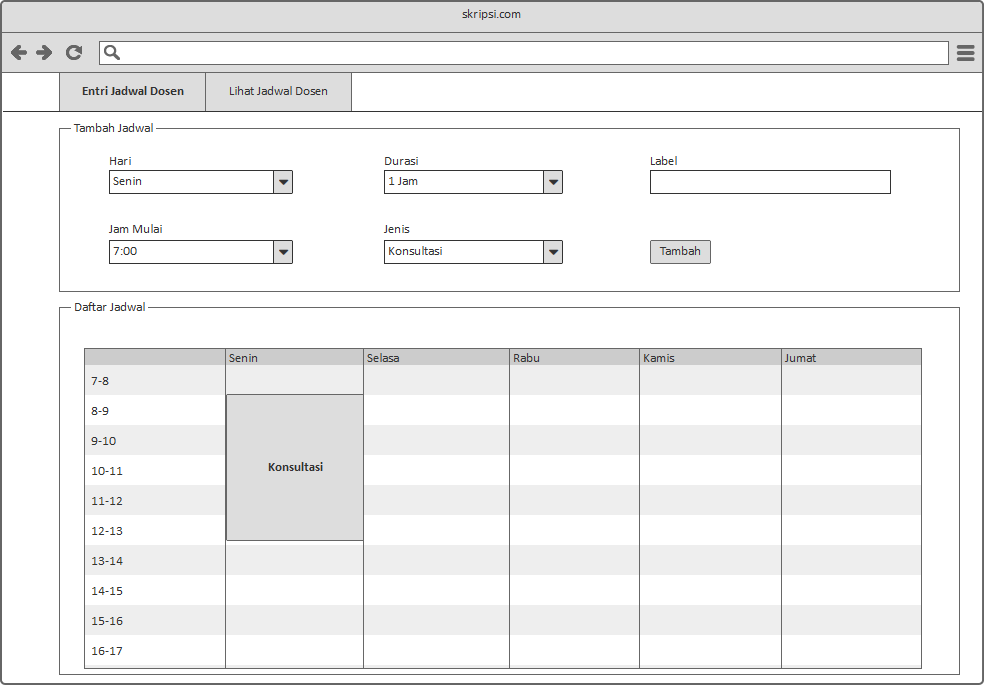
\includegraphics[scale=0.48]{entriJadwalDosen.png}
	\caption[Perancangan Antarmuka Entri Jadwal Dosen]{Perancangan Antarmuka Entri Jadwal Dosen} 
	\label{fig:flow-chart-CodeIgniter} 
\end{figure}
\subsection{Perancangan Antarmuka Edit Jadwal Dosen}
Perancangan antarmuka untuk \textit{pop-up} pengubahan data jadwal yang sudah dimasukan dapat dilihat pada gambar berikut
\begin{figure} [H]
	\centering  
	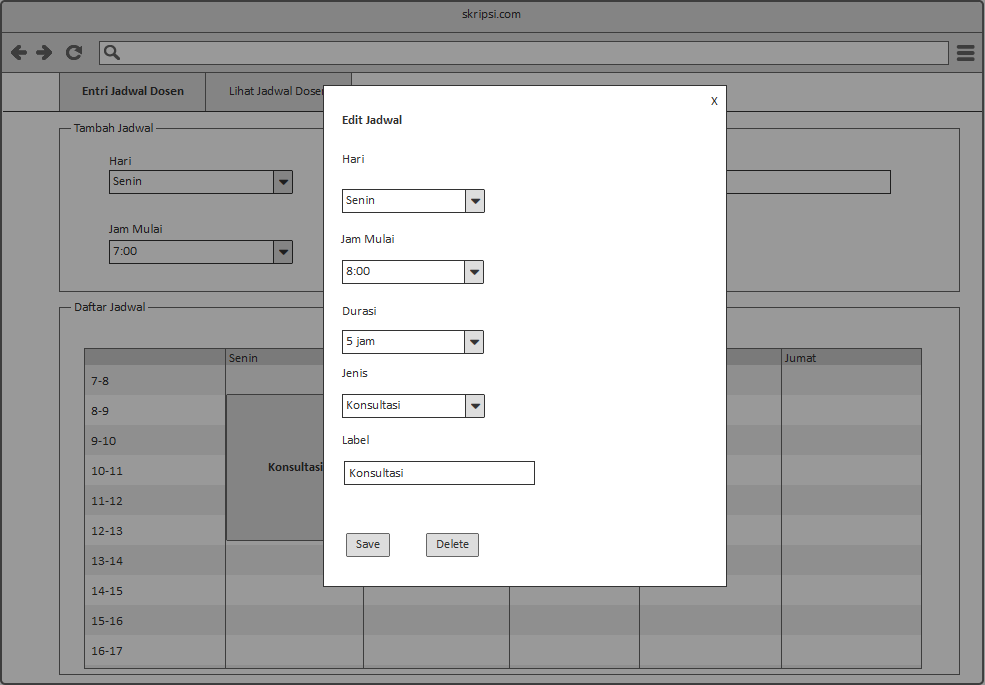
\includegraphics[scale=0.48]{editJadwalModal.png}
	\caption[Perancangan Antarmuka Edit Jadwal Dosen]{Perancangan Antarmuka Edit Jadwal Dosen} 
	\label{fig:flow-chart-CodeIgniter} 
\end{figure}
\subsection{Perancangan Antarmuka Lihat Jadwal Dosen}
Perancangan antarmuka untuk modul Lihat Jadwal Dosen dapat dilihat pada gambar di bawah ini
\begin{figure} [H]
	\centering  
	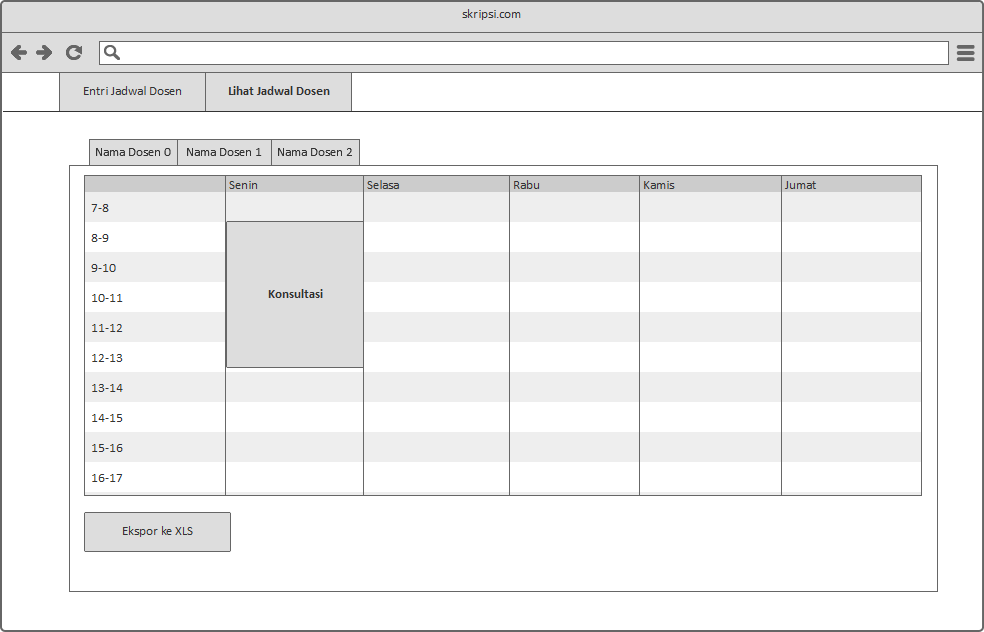
\includegraphics[scale=0.45]{lihatJadwalDosen.png}
	\caption[Perancangan Antarmuka Lihat Jadwal Dosen]{Perancangan Antarmuka Lihat Jadwal Dosen} 
	\label{fig:flow-chart-CodeIgniter} 
\end{figure}